% Snowflake Data Engineering — Chapter 11 | original manuscript draft
% Author: Arman Golbidi | Editorial snapshot: 22 October 2026
% Compile: xelatex -interaction=nonstopmode -halt-on-error Snowflake_Data_Engineering_Chapter_11.tex
% Trim: 178 x 254 mm; margins inside 23 mm / outside 17 mm / top-bottom 19 mm.
% Body: 10.75 pt / 13.65 pt leading = 1.27 line-height ratio; code: 8.75 pt.
\documentclass[11pt,twoside]{article}
\usepackage[paperwidth=178mm,paperheight=254mm,inner=23mm,outer=17mm,top=19mm,bottom=19mm,headheight=5mm,headsep=4mm,footskip=9mm]{geometry}
\usepackage{fontspec}
\setmainfont{LibertinusSerif-Regular.otf}[BoldFont=LibertinusSerif-Bold.otf,ItalicFont=LibertinusSerif-Italic.otf,BoldItalicFont=LibertinusSerif-BoldItalic.otf]
\setsansfont{LibertinusSans-Regular.otf}[BoldFont=LibertinusSans-Bold.otf,ItalicFont=LibertinusSans-Italic.otf]
\setmonofont{LibertinusMono-Regular.otf}[Scale=0.91]
\usepackage[english]{babel}
\usepackage{microtype}
\usepackage{setspace}
\setstretch{1.0}
\usepackage{titlesec,enumitem,tabularx,array,booktabs,needspace,fancyhdr,lastpage}
\usepackage[most]{tcolorbox}
\usepackage{tikz}
\usetikzlibrary{arrows.meta,positioning,fit,shapes.misc,calc}
\usepackage{listings}
\usepackage{xcolor}
\usepackage{hyperref}
\usepackage{amsmath}
\hypersetup{colorlinks=true,urlcolor=steelblue,linkcolor=steelblue,pdfauthor={Arman Golbidi},pdftitle={Snowflake Data Engineering - Chapter 11: Analytics Engineering and Power BI Integration},pdfsubject={English technical book manuscript, eleventh chapter, 178 x 254 mm}}
\definecolor{navy}{HTML}{15334A}
\definecolor{steelblue}{HTML}{17779B}
\definecolor{teal}{HTML}{12888A}
\definecolor{lightblue}{HTML}{ECF5F7}
\definecolor{papergray}{HTML}{F2F5F6}
\definecolor{inkgray}{HTML}{4A5862}
\definecolor{thinrule}{HTML}{CBD7DB}
\AtBeginDocument{\color{navy}\fontsize{10.75}{13.65}\selectfont}
\setlength{\parindent}{0pt}
\emergencystretch=2.5em
\setlength{\parskip}{3.3pt plus 0.7pt minus 0.6pt}
\setlist[itemize]{leftmargin=4mm,itemsep=1pt,topsep=2pt,parsep=0pt}
\setlist[enumerate]{leftmargin=5mm,itemsep=1pt,topsep=2pt}
\titleformat{\section}{\sffamily\bfseries\color{navy}\fontsize{14}{17}\selectfont}{}{0pt}{}
\titlespacing*{\section}{0pt}{8pt}{4pt}
\titleformat{\subsection}{\sffamily\bfseries\color{steelblue}\fontsize{10.8}{13}\selectfont}{}{0pt}{}
\titlespacing*{\subsection}{0pt}{5pt}{1pt}
\newcommand{\topic}[2]{\subsection*{#1\quad #2}}
\newcommand{\repo}[2]{\par\begingroup\fontsize{8.0}{9.6}\selectfont\sffamily\color{inkgray}\textbf{Project reference:} \href{#2}{#1}. \textit{Not independently executed; rights review pending.}\par\endgroup}
\newtcolorbox{insight}[1][]{enhanced,breakable,colback=lightblue,colframe=thinrule,boxrule=.45pt,arc=1.3mm,left=2.8mm,right=2.8mm,top=1.8mm,bottom=1.8mm,before skip=5pt,after skip=5pt,#1}
\newtcolorbox{whitebox}[1][]{enhanced,breakable,colback=papergray,colframe=thinrule,boxrule=.35pt,arc=1mm,left=2.6mm,right=2.6mm,top=1.5mm,bottom=1.5mm,before skip=4pt,after skip=5pt,#1}
\lstdefinestyle{chaptercode}{basicstyle=\ttfamily\fontsize{8.75}{10.7}\selectfont,backgroundcolor=\color{papergray},frame=single,framerule=.35pt,rulecolor=\color{thinrule},breaklines=true,columns=fullflexible,keepspaces=true,showstringspaces=false,aboveskip=5pt,belowskip=5pt,xleftmargin=2mm,xrightmargin=1mm,framexleftmargin=2mm,framexrightmargin=1mm}
\lstset{style=chaptercode}
\pagestyle{fancy}
\fancyhf{}
\fancyhead[LE]{\sffamily\fontsize{7.6}{9}\selectfont\color{inkgray}\textsc{Snowflake Data Engineering}}
\fancyhead[RO]{\sffamily\fontsize{7.6}{9}\selectfont\color{inkgray}\textsc{11 / Power BI \& Analytics}}
\fancyfoot[LE,RO]{\sffamily\bfseries\fontsize{8.2}{9}\selectfont\color{steelblue}\thepage}
\fancyfoot[LO,RE]{\sffamily\fontsize{7.6}{9}\selectfont\color{inkgray}Arman Golbidi \quad | \quad Chapter 11}
\renewcommand{\headrulewidth}{0.35pt}
\renewcommand{\footrulewidth}{0pt}
\setcounter{page}{191}
\raggedbottom

\begin{document}
% PAGE 191
{\sffamily\bfseries\fontsize{9}{11}\selectfont\color{steelblue} CHAPTER 11 \hfill ANALYTICS / TRUSTED CONSUMPTION}\par\vspace{3mm}
{\sffamily\bfseries\fontsize{20.2}{23.4}\selectfont\color{navy} Analytics Engineering\\and Power BI Integration}\par\vspace{2mm}
{\sffamily\fontsize{11.1}{14}\selectfont\color{steelblue} Reliable decisions begin where the pipeline meets the reader}\par\vspace{3mm}
\begin{insight}\textbf{The dashboard is green; the decision is wrong.}\par
An energy team receives a polished visual showing a 66.000~MWh production total. At 08:30 one manager calls that number ``current power'', another treats it as national net supply, and a third compares it with yesterday's demand. Yet the fixture represents one synthetic interval, six technologies, no grid-wide coverage claim, and a separately supplied consumption sample. All three readers can use a technically correct chart to reach a false conclusion. The missing layer is a \emph{contract between data producers and decision makers}.
\end{insight}
Chapters~4 and 10 constructed a dimensional grain and a tested gold transformation. This chapter turns that gold output into a defensible \emph{analytical product}: defined metrics, controlled semantics, documented freshness, deliberate connectivity, usable Power BI reports and an owner who knows what to do when numbers disagree. You will learn not just how to connect a database but how to know whether the resulting report deserves trust.
\begin{whitebox}\textbf{Learning outcomes}\par
After this chapter, you can specify a serving layer; write a versioned KPI contract; configure a read-only Snowflake-to-Power BI connection; choose Import or DirectQuery using measured requirements; plan star-schema and DAX semantics; critique energy dashboard visuals; trace generated queries; establish refresh and incident evidence; and hand off a governed BI product.\end{whitebox}
\textbf{Prerequisites.} Chapters~4--5 and 10, introductory SQL, Power BI terminology, and an understanding of MW versus MWh. The companion includes a \textbf{standard-library Python oracle} and illustrative M/DAX/SQL; there has been \textbf{no live Snowflake or Power BI execution}. Any cloud activity needs approved credentials, a restricted role and a pre-agreed spending limit.
\begin{center}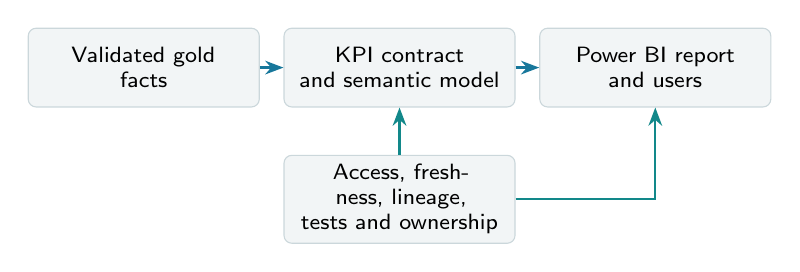
\begin{tikzpicture}[>=Stealth,every node/.style={font=\sffamily\fontsize{7.7}{9}\selectfont},n/.style={draw=thinrule,rounded corners=1mm,fill=papergray,align=center,text width=27mm,minimum height=10mm}]
\node[n](a){Validated gold\\facts}; \node[n,right=3mm of a](b){KPI contract\\and semantic model}; \node[n,right=3mm of b](c){Power BI report\\and users};
\node[n,below=6mm of b](d){Access, freshness, lineage,\\tests and ownership};
\draw[->,thick,steelblue](a)--(b);\draw[->,thick,steelblue](b)--(c);\draw[->,thick,teal](d)--(b);\draw[->,thick,teal](d)-|(c);
\end{tikzpicture}\\{\fontsize{8}{9}\selectfont\color{inkgray}Figure 11.1. A decision is governed across every boundary, not only at ingestion.}\end{center}
\newpage
% PAGE 192
\section*{11.1\quad Analytics engineering and serving-layer design}
\topic{11.1.1}{Serving layer and consumption requirements}
The \emph{serving layer} is the stable interface between engineered data and its consumers. It may consist of governed Snowflake views, materialised tables, a semantic model, APIs or curated extracts. The interface should expose approved fields and business meanings rather than force each report author to reconstruct upstream rules. For our running case, the upstream system resolves source-event revisions and logical deletes before publishing \texttt{FactGeneration} at \emph{one row per UTC interval and technology}. A consumer must never sum the twelve raw delivery rows to calculate production.

A useful serving contract answers five questions: which rows are visible; what is their grain; when is a period complete; which role may access them; and whom should consumers contact after a correction? These questions are more durable than a particular BI product. A Snowflake view can be the public contract; internal bronze tables should not be granted merely to make connector setup easy.
\begin{lstlisting}[language=SQL,caption={Illustrative read-only inspection of the serving grain; not cloud-tested.}]
SELECT interval_utc, technology,
       SUM(energy_mwh) AS generation_mwh
FROM FINLAND_ENERGY_DEMO.GOLD.FCT_ENERGY_HOURLY
GROUP BY interval_utc, technology
ORDER BY interval_utc, technology;
\end{lstlisting}
\topic{11.1.2}{Stakeholder questions and decision support}
A dashboard should begin with a decision, not a chart palette. A grid operator may ask whether observed production balances measured consumption at the \emph{same interval and geographic scope}. A finance analyst may ask for an auditable monthly energy total. An engineering lead may ask whether new source deliveries altered a validated KPI. Those are three different questions, potentially requiring different grains, refresh objectives and ownership.
\begin{center}\renewcommand{\arraystretch}{1.1}\begin{tabularx}{\linewidth}{@{}p{30mm}XX@{}}\toprule
\textbf{Consumer}&\textbf{Question / grain}&\textbf{Acceptance evidence}\\\midrule
Operations&Interval, source scope&Arrival age, coverage and aligned timestamps\\
Finance&Month, approved revisions&Reconciliation and restatement log\\
Engineering&Delivery/run, metric contract&Test status, query ID and lineage\\\bottomrule\end{tabularx}\end{center}
\textbf{Failure case.} A chart titled ``current Finnish electricity supply'' built from our one-interval synthetic fixture invents a scope the source never promised. Replace it with ``Synthetic generation by technology, one UTC interval'' and publish a completeness note.
\repo{P121: Snowflake Labs end-to-end Snowflake and Power BI analytics}{https://github.com/Snowflake-Labs/sfguide-end-to-end-analytics-with-snowflake-and-power-bi}
\textbf{Check.} Which stakeholder question would justify an hourly published mart instead of record-level DirectQuery?
\newpage
% PAGE 193
\topic{11.1.3}{Semantic and physical design responsibilities}
\textbf{Physical design} answers where and how data are stored, partitioned, refreshed and queried. \textbf{Semantic design} defines the user-facing meaning of fields, filter propagation, calculations and hierarchies. The two cooperate but are not interchangeable: accelerating a query does not correct an inconsistent definition of ``renewable share.'' The gold model owns validated revisions and units; the Power BI model owns relationships, visual measures, descriptions and report interactions. The data product owner approves the combined contract.
\begin{center}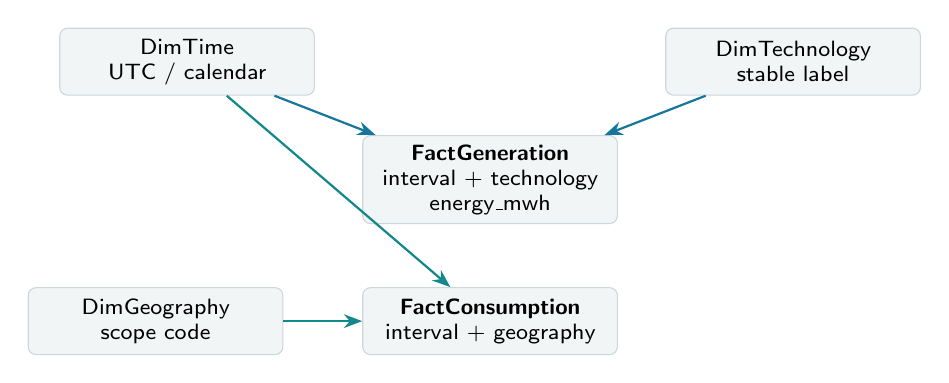
\begin{tikzpicture}[>=Stealth,every node/.style={font=\sffamily\fontsize{7.8}{9}\selectfont},n/.style={draw=thinrule,rounded corners=1mm,fill=papergray,align=center,minimum height=8.5mm,text width=30mm}]
\node[n](f){\textbf{FactGeneration}\\interval + technology\\energy\_mwh};
\node[n,above left=5mm and 6mm of f](t){DimTime\\UTC / calendar};
\node[n,above right=5mm and 6mm of f](d){DimTechnology\\stable label};
\node[n,below=8mm of f](c){\textbf{FactConsumption}\\interval + geography};
\node[n,left=10mm of c](g){DimGeography\\scope code};
\draw[-{Stealth},steelblue,thick](t)--(f);\draw[-{Stealth},steelblue,thick](d)--(f);\draw[-{Stealth},teal,thick](t)--(c);\draw[-{Stealth},teal,thick](g)--(c);
\end{tikzpicture}\\{\fontsize{8}{9}\selectfont\color{inkgray}Figure 11.2. Two separately sourced fact tables share conformed time attributes; they are not directly joined.}\end{center}
\begin{whitebox}\textbf{Who owns which invariant?}\par
\textbf{Snowflake/dbt:} business-key uniqueness, approved revision choice, non-negative energy, source lineage and controlled gold schema. \textbf{Semantic model:} valid relationships, measures, formatting, row-level security where required and report-level context. \textbf{Business owner:} time and geographic comparability, permitted interpretation and metric approval. \textbf{Operations:} refresh health, access review and incident response.\end{whitebox}
A model at the wrong grain is dangerous even when relationships appear valid. Joining \texttt{FactGeneration} directly to \texttt{FactConsumption} on interval alone multiplies the consumption observation once per technology and can inflate totals. Publish \emph{separate measures} and let shared dimensions filter each fact. Validate totals under both single-technology and all-technology selections.

\textbf{Design decision.} Begin with a small, dimensional gold interface and an Import semantic model. Reconsider pre-aggregation or DirectQuery only after observing consumer counts, dataset size, acceptable freshness, query patterns and security obligations. Avoid copying source-derived calculated columns into multiple reports.
\textbf{Check.} Why should consumption not be a column copied onto every technology row?
\newpage
% PAGE 194
\section*{11.2\quad Defining trusted metrics and KPI contracts}
\topic{11.2.1}{Metric definitions, units, and aggregation grain}
A \emph{KPI contract} is an executable promise about a number. It specifies purpose, business grain, formula, numerator, denominator, unit, time basis, expected source completeness, null behaviour, owner, version and permitted aggregation. Without these fields, a report can display mathematically correct but semantically incompatible values.

Our controlled fixture reuses Chapter~10's \emph{six accepted synthetic generation observations}, all at \texttt{2026-03-01T10:00:00Z}: Wind 14, Solar 6, Hydro 18, Nuclear 16, Bioenergy 8 and Other 4~MWh. Their sum is \textbf{66.000~MWh}. This chapter adds \emph{one separately synthetic FI consumption observation} of \textbf{60.000~MWh} at the same UTC interval. The resulting illustrative net position is \textbf{+6.000~MWh}; the wind share of generation is \textbf{14/66 = 21.2121\%}. None is a real Finnish grid statistic.
\begin{center}\renewcommand{\arraystretch}{1.10}\begin{tabularx}{\linewidth}{@{}p{29mm}XX@{}}\toprule
\textbf{KPI}&\textbf{Business rule}&\textbf{Expected fixture}\\\midrule
Generation&Sum accepted MWh at identical scope/interval&66.000 MWh\\
Consumption&Independent, aligned measured MWh&60.000 MWh\\
Net position&Generation $-$ consumption if both present&+6.000 MWh\\
Wind share&Wind / all technologies, equal time/filter context&21.2121\%\\
Source coverage&Observed expected technologies / six&6/6\\\bottomrule\end{tabularx}\end{center}
\begin{insight}\textbf{Power is not energy.}\par
A 480~MW instantaneous or averaged power observation contributes 120~MWh \emph{only if} the measurement represents constant or average power over a 15-minute interval. You cannot add values in MW and label the sum MWh, and you cannot infer a daily energy total from one interval without an explicit coverage assumption.\end{insight}
\textbf{Null is not zero.} An unavailable consumption feed means the net position is \emph{unknown}; rendering zero would create an artificial surplus. Likewise, missing technology should be marked incomplete, not silently treated as valid 0~MWh. The report must distinguish \emph{zero observed} from \emph{not observed}. Use explicit time alignment before subtracting independently provided measures.
\repo{P122: Snowflake Labs dbt semantic view}{https://github.com/Snowflake-Labs/dbt_semantic_view}
\textbf{Check.} Why is the ratio of row-level wind shares not a meaningful daily wind-share KPI?
\newpage
% PAGE 195
\topic{11.2.2}{Ownership and consistency checks}
Metric consistency does not emerge from agreeing on a label. Teams need a \emph{single reviewable definition} and automated checks across layers. The source steward guarantees that timestamps and units are correct, the gold maintainer guarantees one accepted fact per business key, and the BI owner guarantees that a measure respects the intended filter context. A dashboard test should compare the same slice with a direct gold SQL aggregate and an independent oracle.
\begin{lstlisting}[language=SQL,caption={Fixture reconciliation query; illustrative Snowflake relation name.}]
SELECT COUNT(*) AS accepted_rows,
       SUM(energy_mwh) AS generation_mwh
FROM FINLAND_ENERGY_DEMO.GOLD.FCT_ENERGY_HOURLY
WHERE interval_utc =
  '2026-03-01T10:00:00Z'::TIMESTAMP_TZ;
-- Fixture expectation: 6 rows, 66.000 MWh.
\end{lstlisting}
The \emph{identity of the verifier} matters. A DAX measure compared only against another DAX measure sharing the same flawed relationship is not an independent check. Use independently calculated totals, uniqueness tests and negative tests: add a duplicate generation key, omit Solar, supply a negative energy value, or remove consumption. The test should either reject the bad input or render an honest blank/incomplete state. Our companion Python oracle exercises these cases; it does not claim to run DAX.
\topic{11.2.3}{KPI contract changes and review}
Contract evolution is not synonymous with renaming a visual. Suppose stakeholders change ``renewable generation'' to include Bioenergy only when a classification criterion is met. The numerator changes, historical reports may need restatement, and dashboard comparisons become non-equivalent across releases. Approve a new contract version that records the effective date, calculation rule, old/new results, change author and downstream acceptance status.
\begin{whitebox}\textbf{Versioned contract card: \texttt{NET\_POSITION\_MWH / v0.1}}\par
\textbf{Formula:} aligned generation MWh minus aligned consumption MWh. \textbf{Grain:} UTC interval and common geographic scope. \textbf{Missing data:} return blank and raise a completeness note. \textbf{Owners:} grid-source steward and analytics product owner. \textbf{Change gate:} two-person review, fixture reconciliation, DAX check, visual caption review and release note.\end{whitebox}
When the calculation changes, update \texttt{metrics\_catalogue.md}, semantic model documentation, tests, downstream contracts and training examples in the same reviewed pull request. Do not silently update a production measure while leaving a dashboard title unchanged. Consider using Snowflake semantic views or dbt metric infrastructure where appropriate, but compare feature support and governance boundaries rather than assuming tools enforce business meaning automatically.
\repo{P123: Snowflake Labs semantic-model-generator}{https://github.com/Snowflake-Labs/semantic-model-generator}
\textbf{Check.} What evidence would prove that a contract change preserves comparability with the previous monthly series?
\newpage
% PAGE 196
\section*{11.3\quad Snowflake connectors and BI integration}
\topic{11.3.1}{Supported Snowflake connectivity}
A connector is more than a connection string: it selects a driver, an authentication route, a source role, a compute warehouse, a query mode and a refresh behaviour. The maintained \emph{Power Query Snowflake connector} supports Import and DirectQuery for Power BI semantic models. Microsoft documents connector implementation~2.0 using an Arrow Database Connectivity (ADBC) driver, with new Power BI Desktop connections using this implementation by default; existing installations and the host version still matter. Check the actual release notes before production rather than hard-coding an assumption about a particular tenant.
\begin{lstlisting}[caption={Power Query M connection template; not run in Power BI.}]
Source = Snowflake.Databases(
  "YOUR_ACCOUNT_IDENTIFIER.snowflakecomputing.com",
  "BI_WH", [Implementation="2.0", Role="BI_READER"]
)
\end{lstlisting}
This is a \emph{template}, not a turnkey credential. Replace the account host, select a permitted warehouse and verify the exact role and navigator paths in the installed Desktop version. The Power Query dialog normally asks for a Snowflake server and warehouse and provides a choice of storage mode. Always verify which objects Power BI is permitted to discover; prefer curated Gold views or tables instead of raw sensitive layers.
\topic{11.3.2}{Credential and gateway considerations}
Common enterprise authentication patterns include named credentials, approved Microsoft Entra integration and key-pair/service-principal arrangements where supported by the product and connector combination. Authentication capability varies by connector implementation and cloud deployment. Never paste credentials into a PBIX, an M file, Git history or a screenshot. Keep account secrets in organisation-approved credential facilities and rotate them by policy.
\begin{center}\renewcommand{\arraystretch}{1.08}\begin{tabularx}{\linewidth}{@{}p{31mm}X@{}}\toprule
\textbf{Boundary}&\textbf{Required review}\\\midrule
Power BI Desktop&Connector version, allowed account and local sign-in\\
Power BI Service&Stored credentials/SSO, capacity and refresh settings\\
Snowflake&Role grants, BI warehouse, object exposure and query logs\\
Network/gateway&Cloud connectivity, proxy/private route, gateway only if required\\\bottomrule\end{tabularx}\end{center}
\textbf{Avoid a generic gateway assumption.} The Snowflake cloud connection can often run without an on-premises gateway; enterprise networking, private endpoints or organisation-specific topology may change that. Test the \emph{actual published-service connection}, not only Desktop success.
\repo{P124: snowflakedb/snowflake-connector-net}{https://github.com/snowflakedb/snowflake-connector-net}
\textbf{Check.} Which four values should an operator record when a published refresh fails despite working on the developer's machine?
\newpage
% PAGE 197
\topic{11.3.3}{Refresh, user identity, and permissions}
Credential success does not prove that the right person is querying the right rows. Power BI workspace membership controls who can interact with a report; semantic model permissions and optional Power BI row-level security (RLS) govern model visibility; Snowflake roles govern the upstream objects. Their policies can diverge. In \emph{Import}, the configured refresh identity retrieves data into the model, and downstream user filtering is primarily enforced within the published semantic model. In \emph{DirectQuery}, report queries reach Snowflake; without supported single sign-on (SSO), a configured identity can serve many viewers. With correctly configured Microsoft Entra SSO, the end user's identity can be delegated for the supported DirectQuery path. Never imply that SSO is automatic.

Grant a reader role only \texttt{USAGE} on the approved database, schema and warehouse and \texttt{SELECT} on curated Gold objects. Keep data engineering write roles separate. Confirm the account's actual grants and ownership; do not provide a blanket privileged role to sidestep a login issue.
\begin{lstlisting}[language=SQL,caption={Review queries for a permitted reviewer; illustrative.}]
SELECT CURRENT_ROLE(), CURRENT_WAREHOUSE();
-- As an authorised administrator/reviewer only:
SHOW GRANTS TO ROLE BI_READER;
-- Inspect approved grants, not raw credentials.
\end{lstlisting}
\begin{insight}\textbf{Security test: two real identities, two expected views.}\par
A source-owner account might see all approved rows while a restricted reader should see only their authorised slice. Test the actual published report with both identities, not a single developer account impersonating the other without recording evidence. When SSO is unavailable, design compensating semantic-model RLS and verify it explicitly.\end{insight}
For published refreshes, log at least the model name, run start/end, source readiness timestamp, status, changed row counts, failed stage and owner. DirectQuery may not need an Import refresh but still relies on up-to-date source transformations, warehouse availability and report cache behaviour. A report click may reuse a prior result; observing a visual refresh is not proof of instantaneous source propagation.

Connector migration notes document implementation-specific issues. Check distinct counts and large-model loads with the installed driver; one benchmark does not establish universal correctness or performance.
\repo{P125: Snowflake Labs marketplace-data-app}{https://github.com/Snowflake-Labs/sfguide-marketplace-data-app}
\textbf{Check.} Where would you enforce regional visibility if all DirectQuery consumers share one stored Snowflake identity?
\newpage
% PAGE 198
\section*{11.4\quad Power BI Import and DirectQuery considerations}
\topic{11.4.1}{Import versus DirectQuery trade-offs}
\textbf{Import} stores a compressed copy inside the Power BI semantic model and queries that cache interactively. \textbf{DirectQuery} leaves the bulk of source data in Snowflake and sends one or more source queries as users interact. Neither means ``always fast'' or ``always current''. Import depends on refresh; DirectQuery depends on source completion, latency, security, caching and the frequency of visual queries. Microsoft generally recommends starting with Import, then justifying alternatives using requirements.
\begin{center}\renewcommand{\arraystretch}{1.13}\begin{tabularx}{\linewidth}{@{}p{26mm}XX@{}}\toprule
\textbf{Dimension}&\textbf{Import}&\textbf{DirectQuery}\\\midrule
Typical visual work&Power BI engine&Snowflake and connector\\
Source change&Visible after model refresh&Visible after subsequent query/cache refresh\\
Model capacity&Memory/storage for data&Remote query and concurrency cost\\
Semantics&Flexible modelling&DAX / transformation restrictions\\
Security&Model RLS and refresh identity&Source SSO only if configured; otherwise shared identity\\\bottomrule\end{tabularx}\end{center}
\topic{11.4.2}{Model size, latency, and costs}
For Import, evaluate row count, compressed model size, refresh duration, memory, licence limits and historical retention. For DirectQuery, evaluate concurrent viewers, per-page visuals, interaction count, SQL shape, warehouse warm-up, queueing, result caching and cost. More visuals and slicer changes can multiply source queries. No performance estimate follows from our six-row fixture.
\topic{11.4.3}{Choosing a mode for energy data}
If daily operational reporting tolerates periodic refresh, a small Gold aggregate in Import is a defensible baseline. If a control-room report needs a verified sub-refresh freshness requirement and cannot meet it with Import/incremental refresh, evaluate DirectQuery, a hybrid arrangement or another platform design. Beware of calling every fast-updating panel ``real time'': document \emph{event-time lag}, \emph{source-ready lag}, \emph{model lag} and \emph{visual display lag} separately.
\begin{whitebox}\textbf{Architecture decision BI-011 (illustrative)}\par
\textbf{Chosen starting mode:} Import of a restricted Gold mart. \textbf{Reason:} predictable historical chart interaction and simple operational checks. \textbf{Open risks:} refresh schedule, model limits and business-approved SLA are unverified. \textbf{Revisit:} when measured data freshness, storage or concurrency breaks acceptance criteria.\end{whitebox}
\repo{P126: mattfeks/Snowflake-PowerBI}{https://github.com/mattfeks/Snowflake-PowerBI}
\textbf{Check.} Why might a ten-second cold DirectQuery visual cost more and feel worse than an hourly Import model, even with identical Snowflake data?
\newpage
% PAGE 199
\section*{11.5\quad Semantic modelling and refresh strategies}
\topic{11.5.1}{Dimensional relationships and DAX semantics}
In the semantic model, define a \emph{dimension-to-fact} filter path with stable keys, explicit single-direction relationships and intentionally named measures. \texttt{FactGeneration} relates to technology and time dimensions; a separate consumption fact relates to time and geography. Do not connect facts directly or enable bidirectional filtering simply because a total looks wrong. \emph{DAX filter context} determines which rows a measure sees; a card, slicer and bar chart can therefore evaluate the same measure at different slices.
\begin{lstlisting}[caption={Illustrative DAX, not evaluated by the offline tests.}]
Generation MWh = SUM('FactGeneration'[energy_mwh])
Consumption MWh =
  SUM('FactConsumption'[consumption_mwh])
Net Position MWh =
  IF(ISBLANK([Generation MWh]) ||
     ISBLANK([Consumption MWh]), BLANK(),
     [Generation MWh]-[Consumption MWh])
\end{lstlisting}
A ratio such as wind share needs a clearly defined denominator. If the dashboard filters technology to Wind, \texttt{Generation MWh} returns 14~MWh; for an ``overall wind share'' tile, the denominator must remove \emph{only} the technology filter while retaining compatible time/geography filters. Never sum per-technology percentages or use a cross-region denominator by accident.
\topic{11.5.2}{Dataset refresh frequency}
The fastest available refresh schedule is not necessarily the appropriate one. Start with the business decision deadline, source publication cycle and data delivery quality. An Import model refreshed every 15 minutes does not become current if Snowflake gold is updated only every two hours. Capacity, licence, incremental-refresh policy, service limits and gateway topology may constrain frequency; verify these in the target environment rather than promising a fixed universal limit.
\topic{11.5.3}{Freshness and lineage validation}
Record a chain of evidence: latest expected source event timestamp $\to$ accepted Gold publication timestamp $\to$ last successful semantic-model refresh $\to$ last visual evaluation. A green refresh indicator means a refresh ran; it does not prove that a source delivered recent or complete data. Every operational report should expose its \emph{as-of} timestamp and data coverage status.
\begin{insight}\textbf{Missing consumption rule.}\par
If the consumption record disappears, the correct net KPI is \emph{blank/unknown}, not +66~MWh. The offline lab asserts this as a contract rule.\end{insight}
\repo{P128: snowflake-semantic-views-powerbi}{https://github.com/alexfrancisross/snowflake-semantic-views-powerbi}
\textbf{Check.} Why does a DAX grand total often need reevaluation of the measure rather than summing displayed row percentages?
\newpage
% PAGE 200
\section*{11.6\quad Building energy analytics dashboards}
\topic{11.6.1}{Generation and consumption KPIs}
A useful energy dashboard presents \emph{unit, period, scope and completeness} before a striking number. Our synthetic report begins with four cards: generation \textbf{66.000~MWh}, consumption \textbf{60.000~MWh}, net position \textbf{+6.000~MWh}, and source-technology coverage \textbf{6/6}. A footnote makes clear that generation and consumption are different synthetic inputs aligned for a single UTC interval. These are teaching fixtures, not observed national production or demand.
\topic{11.6.2}{Meaningful visuals and filters}
Use a horizontal bar chart for the six technology values: Hydro 18, Nuclear 16, Wind 14, Bioenergy 8, Solar 6 and Other 4~MWh. Zero-based bars and explicit MWh labels support comparison. Add technology, UTC time and source-scope selectors only if the underlying model actually supports their values. A trend line needs multiple timestamps; one data point is not a trend, and a synthetic extension must be labelled as such.
\begin{center}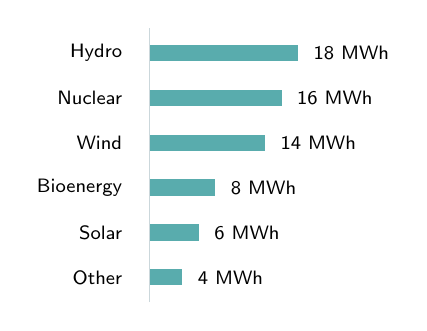
\begin{tikzpicture}[x=.105cm,y=.57cm,every node/.style={font=\sffamily\fontsize{7.5}{8.8}\selectfont}]
\foreach \name/\val/\j in {Hydro/18/5,Nuclear/16/4,Wind/14/3,Bioenergy/8/2,Solar/6/1,Other/4/0}{
\node[anchor=east] at (-2.1,\j){\name};
\fill[teal!70] (0,\j-.18) rectangle (\val,\j+.18);
\node[anchor=west] at (\val+.7,\j){\val\ MWh};
}
\draw[thinrule] (0,-.55)--(0,5.55);
\end{tikzpicture}\\{\fontsize{8}{9}\selectfont\color{inkgray}Figure 11.3. Original illustration of the controlled six-technology synthetic snapshot.}\end{center}
\topic{11.6.3}{Interpretation cautions and data completeness}
Every chart should answer ``what is excluded?'' The six-technology fixture does not establish complete Finnish generation coverage, imports/exports, transmission loss, or the scope of actual measurement providers. A high visual completion score for \emph{expected fixture technologies} must not be presented as nationwide data quality. Add an \emph{as-of} label, dataset identifier, last source success, known exclusions and a short link to definitions.
\begin{whitebox}\textbf{Dashboard acceptance checklist}\par
Accurate title and units; aligned UTC time; accessible colours and readable labels; no false precision; tested slice totals; visible missing-data state; filter instructions; and documented source, owner and release version.\end{whitebox}
\repo{P129: Customer Insights with Snowflake and Power BI (community reference)}{https://github.com/BalajiKottana/Customer_Insights_with_Snowflake_and_PowerBI}
\textbf{Check.} Which two annotations would prevent our six-bar chart from being mistaken for a national energy-mix estimate?
\newpage
% PAGE 201
\section*{11.7\quad Dashboard performance and query behaviour}
\topic{11.7.1}{Generated SQL and pushdown behaviour}
Query performance begins at the consumption boundary. A Power BI visual translates an analytical request into DAX and, in DirectQuery mode, typically sends native queries to Snowflake. The database may see multiple generated SQL statements for one visual interaction. \emph{Query folding} means eligible Power Query operations are delegated to the source rather than processed inefficiently after data retrieval. For DirectQuery tables, scalable folding is essential; for Import, folding can reduce refresh cost and transfer size.

For a six-category bar chart, a source-side grouping is natural. This SQL is \emph{illustrative of the intended result}, not a claim about the exact SQL a specific connector build generates:
\begin{lstlisting}[language=SQL,caption={Expected pushdown shape for a grouped visual.}]
SELECT technology, SUM(energy_mwh) AS generation_mwh
FROM FINLAND_ENERGY_DEMO.GOLD.FCT_ENERGY_HOURLY
WHERE interval_utc =
  '2026-03-01T10:00:00Z'::TIMESTAMP_TZ
GROUP BY technology;
\end{lstlisting}
\begin{center}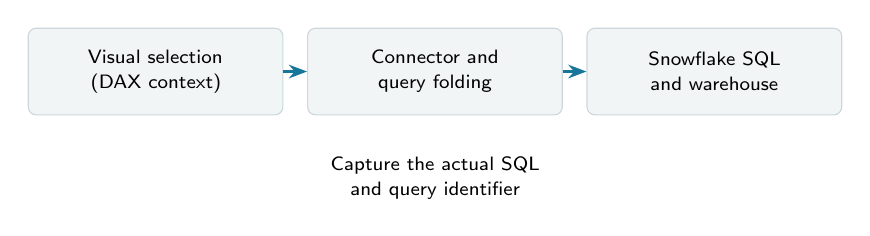
\begin{tikzpicture}[>=Stealth,every node/.style={font=\sffamily\fontsize{7.5}{9}\selectfont},n/.style={draw=thinrule,rounded corners=1mm,fill=papergray,align=center,text width=30mm,minimum height=11mm}]
\node[n](a){Visual selection\\(DAX context)};
\node[n,right=3mm of a](b){Connector and\\query folding};
\node[n,right=3mm of b](c){Snowflake SQL\\and warehouse};
\draw[->,thick,steelblue](a)--(b);\draw[->,thick,steelblue](b)--(c);
\node[below=4mm of b,align=center,text width=41mm]{Capture the actual SQL and query identifier};
\end{tikzpicture}\\{\fontsize{8}{9}\selectfont\color{inkgray}Figure 11.4. The generated query is evidence, not a guess from a visual's appearance.}\end{center}
\textbf{A folding trap.} Complex custom functions, certain native SQL patterns and transformations after a native query can prevent efficient folding. Microsoft guidance warns that DirectQuery native SQL inputs have restrictions and that incremental refresh depends on compatible folding. Prefer validated Gold views for complex source logic. Use the installed Power Query folding indicators and Performance Analyzer to inspect real behaviour.
\textbf{Check.} If a visual performs well with six rows but stalls with six million, which evidence distinguishes bad SQL pushdown from BI visual rendering overhead?
\newpage
% PAGE 202
\topic{11.7.2}{Performance troubleshooting}
Do not fix a slow report by blindly increasing the Snowflake warehouse size. First reproduce a single interaction with a specific dataset, user role, filter state and connector version. Measure the time users experience, then separate Power BI visual rendering, DAX calculation, network latency, Snowflake compilation, queueing and execution. Power BI Performance Analyzer and Snowflake Query History/Query Profile provide complementary views. Each measurement needs a timestamp, relevant identifiers and a cache-state note.
\begin{center}\renewcommand{\arraystretch}{1.12}\begin{tabularx}{\linewidth}{@{}p{32mm}XX@{}}\toprule
\textbf{Observed symptom}&\textbf{Possible mechanism}&\textbf{First evidence}\\\midrule
First click slow, next quick&Warehouse wake-up or cache&Resume time and profile\\
Slicer creates long waits&Excess source round trips&Analyzer query counts\\
Slow despite small result&Poor pruning or big join&SQL text and profile\\
Peak-hour timeouts&Concurrency/queueing&Warehouse load and history\\
Refresh uses excess memory&Connector/model processing&Refresh log, driver version\\\bottomrule\end{tabularx}\end{center}
A valid experiment holds dataset, filter set, user role and output semantics constant. Run repeated controlled trials and report medians or percentiles with sample sizes. Compare warm and cold behaviour separately; querying a cached six-row result is not a general Snowflake benchmark. Include warehouse time in any cost comparison and document what was actually billed. The companion package does \emph{not} provide fabricated p95 latency or credit consumption.

Power BI modelling decisions affect source load: high-cardinality joins, ambiguous relationships, broad \texttt{DISTINCTCOUNT}, cross-highlighting and too many simultaneously refreshing visuals can increase query complexity. Source-side aggregation often helps, but must preserve correct filter semantics. A pre-aggregated table that drops the technology key cannot correctly answer a technology-specific question. Compare a candidate aggregate against the detailed gold model under representative filters before making it the default.
\begin{insight}\textbf{Cost optimisation that silently changes the answer is not an optimisation.}\par
The acceptance benchmark is \emph{same users, same filter context, same valid rows, same KPI contract, comparable cache and warehouse settings}. Make correctness the first gate and latency/cost the second.\end{insight}
\repo{P132: streamlit-page-analytics (related app measurement reference)}{https://github.com/Snowflake-Labs/streamlit-page-analytics}
\textbf{Check.} Why is comparing Import card response time with cold-start DirectQuery time without reporting mode a misleading benchmark?
\newpage
% PAGE 203
\topic{11.7.3}{Refresh reliability and user-perceived delay}
A semantic model can report \emph{refresh succeeded} while the information a human sees is stale. Separate four clocks: $t_s$ is the event interval, $t_g$ is the timestamp when approved Gold was ready, $t_r$ is the last successful model refresh and $t_v$ is when the visual was actually evaluated. An end-user freshness delay can be described as $t_v-t_s$ \emph{only if} the displayed data correspond to event time $t_s$ and every intervening state is known.
\[
\text{Source-to-gold age}=t_g-t_s,\qquad
\text{Gold-to-model delay}=t_r-t_g.
\]
These are explanatory measurements, not guaranteed service-level agreements. In DirectQuery, a fresh interaction may query source data directly, but caching and source completion still matter. In Import, a model refresh defines when changes can become visible, and tiles or browser sessions can retain other cached states.
\begin{center}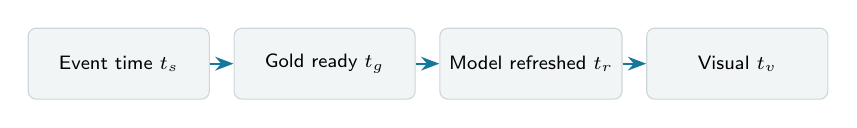
\begin{tikzpicture}[>=Stealth,every node/.style={font=\sffamily\fontsize{7.5}{8.5}\selectfont},n/.style={draw=thinrule,rounded corners=1mm,fill=papergray,align=center,minimum width=23mm,minimum height=9mm}]
\node[n](a){Event time $t_s$};\node[n,right=3mm of a](b){Gold ready $t_g$};\node[n,right=3mm of b](c){Model refreshed $t_r$};\node[n,right=3mm of c](d){Visual $t_v$};
\draw[->,steelblue,thick](a)--(b);\draw[->,steelblue,thick](b)--(c);\draw[->,steelblue,thick](c)--(d);
\end{tikzpicture}\\{\fontsize{8}{9}\selectfont\color{inkgray}Figure 11.5. Preserve each timestamp to diagnose which boundary became stale.}\end{center}
\begin{whitebox}\textbf{An illustrative failure walk-through}\par
At 08:00, Gold still reflects events up to 06:00. An Import refresh at 08:05 succeeds and stamps \emph{08:05 refresh success}; the report opened at 08:10 still contains no events after 06:00. The correct operator response is to investigate source lateness, not force repeated Power BI refreshes.\end{whitebox}
Set freshness and availability targets from an approved operational requirement, and alert separately on missed upstream arrivals, failed transformations, failed model refresh, invalid KPI reconciliation and inaccessible reports. Record the incident's \emph{first affected period}, not only the first visible error. After recovery, compare corrected output and downstream caches; do not silently backfill without a restatement note when user-facing historical values change.

\textbf{Check.} What two timestamps would you request first if a Power BI model refreshed at 09:00 but the dashboard still shows yesterday's energy values?
\newpage
% PAGE 204
\section*{11.8\quad Data-sharing patterns and operational handoff}
\topic{11.8.1}{Governed sharing and access policies}
Sharing a report is not the same as sharing unrestricted access to source data. Distribution choices include Power BI workspace/apps, governed semantic models, approved Snowflake views and Snowflake secure data-sharing capabilities. Each moves a different boundary. A Power BI report user may only need permission to view a published report, while a Snowflake data consumer may need a dedicated reader role and object grants. Source permissions, personal-data scope, regional restrictions and retention rules must be checked before choosing the channel.

For the energy case, expose a read-only Gold interface for approved analysts and distribute visual consumption through the BI workspace. If other teams need curated tables directly, use dedicated grants or an approved governed sharing mechanism. Never make a raw ingestion schema public merely because a BI connector can see it. If row-level visibility differs between departments, coordinate Snowflake row access policies, model RLS and source identity; do not rely on workspace visibility alone.
\begin{center}\renewcommand{\arraystretch}{1.12}\begin{tabularx}{\linewidth}{@{}p{33mm}XX@{}}\toprule
\textbf{Audience}&\textbf{Allowed surface}&\textbf{Security decision}\\\midrule
Executive reader&Published report&Viewer access and approved model RLS\\
BI developer&Development Gold interface&Least-privilege Snowflake role\\
Data engineer&Controlled source and test data&Separate write role, audit logging\\
External consumer&Governed sharing product&Contract, classification and approval\\\bottomrule\end{tabularx}\end{center}
\begin{insight}\textbf{Data residency is not proven by placing Snowflake in one region.}\par
Power BI tenant/capacity settings, exports, caches, user downloads, support operations and any external connections also matter. A compliance claim requires review of the complete flow and the organisation's applicable obligations, not just one region selector.\end{insight}
Before releasing a report, inspect every field exposed in the semantic model, including hidden technical columns that might be accessible through alternate report or export paths. Validate exports, workspace sharing and any Build permissions. Apply sensitivity labels and audit policies where applicable, but verify their enforcement in the configured tenant.
\repo{P133: Snowflake Labs Horizon intra-organisation sharing}{https://github.com/Snowflake-Labs/sfguide-horizon-intra-organization-sharing}
\textbf{Check.} Why can a report be correctly protected in Power BI while a shared Snowflake reader role remains over-permissive?
\newpage
% PAGE 205
\topic{11.8.2}{Report documentation and ownership}
An analytical product needs a human maintenance story. Its README should name a product owner, a technical maintainer and a source steward, then state the metric contract version, Gold objects, refresh mode, normal freshness window, row-level permission model, dependencies and escalation route. Add a report change log, dashboard screenshots with capture dates, and an explicit note about data coverage. \emph{No one owns it} is an architectural defect, not a documentation nicety.
\begin{whitebox}\textbf{Suggested report manifest (example)}\par
\textbf{Name:} Finland Energy Analytics / Synthetic Demonstrator. \textbf{Source:} approved Gold generation + separately supplied synthetic consumption. \textbf{Grain:} UTC interval and technology, or interval and geography. \textbf{Mode:} proposed Import, pending tenant approval. \textbf{KPI version:} 0.1. \textbf{Owner:} analytics product owner (to be assigned). \textbf{Runbook:} section 11.8.3. \textbf{Release state:} design and offline tests only.\end{whitebox}
Every measure should carry a plain-language description, unit, aggregation restrictions, empty-data handling and the exact version of the upstream contract on which it depends. Provide a curated field list with intended slicers, relationships and hidden columns. The \texttt{semantic\_model\_spec.md} and \texttt{metrics\_catalogue.md} companion files are examples of this handoff. They are design documents, not exports from a completed Power BI semantic model.

Lineage should be bidirectional: a reader can trace ``Net Position MWh'' back through DAX, two fact tables, Gold business rules, source intervals and synthetic fixtures; an operator can trace a changed source contract forward into dependent measures, reports and users. Store accountable links and version tags, not only screenshots of a graph. Avoid an opaque multi-report chain in which the final business definition depends on undocumented intermediate calculated columns.
\begin{center}\renewcommand{\arraystretch}{1.10}\begin{tabularx}{\linewidth}{@{}p{38mm}X@{}}\toprule
\textbf{Documentation artifact}&\textbf{Maintenance purpose}\\\midrule
KPI catalogue&Business meaning, formulas, effective dates\\
Semantic model spec&Grain, keys, filter paths, DAX decisions\\
Refresh/runbook&Failure steps and authorised recovery\\
Release log&What changed, proof and rollback reference\\
Access matrix&Who sees which data, reviewed by whom\\\bottomrule\end{tabularx}\end{center}
\textbf{Check.} Which artifact would you consult first if Finance claims the net position changed after a model release but no source delivery changed?
\newpage
% PAGE 206
\topic{11.8.3}{Operational acceptance and maintenance}
A handoff is complete when a second operator can detect, explain and recover from a failure \emph{without guessing the designer's intentions}. Before release, a reviewer should validate Gold row-grain uniqueness, KPI totals, missing-data behaviour, SSO/RLS boundaries, refresh schedules, user-visible freshness and dashboard accessibility. Then rehearse one failure: suspend the BI warehouse or block the test source in a disposable environment, confirm the alert, restore only approved resources and demonstrate that the downstream result is correct.
\begin{center}\renewcommand{\arraystretch}{1.10}\begin{tabularx}{\linewidth}{@{}p{33mm}XX@{}}\toprule
\textbf{Incident signal}&\textbf{Evidence to collect}&\textbf{First safe response}\\\midrule
Missing expected KPI&Contract, source coverage&Freeze distribution; trace lineage\\
Permission denied&Identity, role, workspace&Review grants; no admin bypass\\
Unexpected stale data&Last source/Gold/model times&Fix failing stage, then refresh\\
Slow report&Analyzer and Query Profile&Reproduce before resizing\\
Wrong value after release&Metric version, independent oracle&Rollback semantic change if approved\\\bottomrule\end{tabularx}\end{center}
\begin{insight}\textbf{Rollback is a controlled data-product operation.}\par
Reverting a DAX measure or report is different from undoing a Gold transformation. Keep source history and prior approved metric contract. Do not drop a production database, delete valid event history or claim a blanket \texttt{DROP} is a safe cleanup strategy. For an actual tenant, use the organisation's version-control and deployment pipeline.\end{insight}
Define a \emph{stop-the-line} gate for critical incidents: broken RLS, incorrect unit, duplicated current key, leaked fields or materially wrong KPI. An attractive visual with such a defect is not fit for decision support. Conversely, a minor label adjustment may follow a lightweight change path if the owner approves and regression tests pass.

Acceptance evidence should include the precise environment, semantic model and connector versions; the approved report or PBIP/PBIX artifact; the dataset version and query/refresh IDs; redacted screenshots; tests of at least two identities; source reconciliation; and the signed handoff checklist. Our laboratory cannot supply live proof for these items and explicitly records that limitation.
\repo{P134: Snowflake Labs internal marketplace sharing}{https://github.com/Snowflake-Labs/sfguide-intra-company-data-sharing-with-the-snowflake-internal-marketplace}
\textbf{Check.} When an upstream correction changes yesterday's KPI, who authorises the restatement and what evidence tells users it happened?
\newpage
% PAGE 207
\section*{11.L\quad Guided lab, chapter review, and exercises}
\topic{11.L.1}{Prerequisites, inputs, environment, permissions, and cost guardrails}
\textbf{Scenario.} Extend the Chapter~10 gold energy output into a reviewable reporting contract. The primary fixture has six synthetic generation rows totalling \textbf{66.000 MWh} at \texttt{2026-03-01T10:00:00Z}. A \emph{separate artificial consumption fixture} contains one FI observation at the same UTC interval, \textbf{60.000 MWh}. Neither constitutes an actual Finnish energy dataset. The goal is to specify a Power BI semantic model, document a dashboard and verify the measures offline before anyone authenticates to Snowflake or Power BI.

\textbf{Files.} The companion lab includes generation and consumption CSVs; \texttt{metrics.py} and tests; a KPI catalogue; a semantic model specification; DAX, M and SQL templates; and a report README. The Power BI folder is a \emph{design package}, not a finished \texttt{.pbix}.

\textbf{Offline prerequisite.} Python 3.10+ and a local terminal; no external dependencies, Snowflake credits or Power BI subscription. \textbf{Optional cloud stage.} A current Power BI Desktop installation, approved Snowflake account, read-only BI role and auto-suspending small warehouse. Record estimated cost, responsible approver and cleanup scope before cloud access. Do not run a chargeable environment merely to validate six rows.
\topic{11.L.2}{Step-by-step procedure with selected code and expected results}
\begin{enumerate}
\item Run the offline contract oracle and all tests. Keep its machine-readable output.
\item Inspect grain and keys; verify six unique generation rows and one aligned consumption record.
\item Review \texttt{metrics\_catalogue.md} and challenge the distinction between MWh and MW, blank and zero, fixture coverage and national scope.
\item Draw the proposed dimensional relationships, write DAX measures, and review the dashboard page specification. For a real report, build it manually in Desktop and retain the resulting PBIX/PBIP plus screenshots.
\item If separately approved, point the template at a disposable Snowflake Gold environment, inspect Power Query folding and query history, then verify refresh and access with authorised identities. This step is \textbf{not} recorded as completed.
\end{enumerate}
\begin{lstlisting}[caption={Zero-cloud command sequence from the companion lab.}]
cd lab
python metrics.py
python -m unittest discover -s tests -v
# All source/account credentials are optional and separate.
\end{lstlisting}
\begin{whitebox}\textbf{Offline fixture oracle}\par
\textbf{Generation:} 66.000~MWh. \textbf{Consumption:} 60.000~MWh. \textbf{Net:} +6.000~MWh. \textbf{Wind share:} $14/66\approx21.2121\%$. \textbf{Accepted technologies:} 6/6. These are exact fixture calculations; they do \emph{not} test Snowflake, DAX, Power BI rendering or refresh latency.\end{whitebox}
\newpage
% PAGE 208
\topic{11.L.3}{Expected result, assertions, common failure diagnosis, rollback, and cleanup}
A pass must validate exact fixture totals, non-negative finite MWh, one row per generation key, aligned UTC timestamps, allowed technologies, separate consumption grain and \emph{blank net position} when consumption is absent. The accompanying test suite also injects duplicate and negative records, unexpected technology, non-UTC time, missing technology and duplicate consumption; each must be rejected or handled explicitly. Only the Python fixture semantics have been executed; the M and DAX files are templates that require independent product-specific validation.
\begin{center}\renewcommand{\arraystretch}{1.1}\begin{tabularx}{\linewidth}{@{}p{31mm}X@{}}\toprule
\textbf{Symptom}&\textbf{Investigate first}\\\midrule
Total $\neq66$ MWh&Wrong revision, duplicate key or filter context\\
Net equals generation&Consumption missing or blank incorrectly coerced to zero\\
Visual unexpectedly slow&Query mode, folding, generated SQL and cold start\\
Refresh green, data stale&Source-ready time versus model refresh time\\
Restricted user sees all&Stored credentials, RLS, SSO and Snowflake grants\\\bottomrule\end{tabularx}\end{center}
\textbf{Rollback and cleanup.} Remove the locally generated metrics JSON to reset the offline lab. The SQL examples are read-only. For any approved cloud exercise, suspend the learner-owned warehouse and follow an authorised cleanup checklist; never modify shared production objects.
\topic{11.L.4}{Foundation exercise, practitioner exercise, production-design question, and scoring rubric}
\textbf{Foundation (20 points):} explain fact grains and compare Import with DirectQuery. \textbf{Practitioner (35):} remove consumption to prove net is unknown; add a second synthetic interval and update trend tests. \textbf{Architecture (30):} design a restricted BI connection with freshness and incident rules. \textbf{Evidence (15):} provide logs, KPI catalogue, model spec and untested-cloud limitations. \emph{Pass:} 80/100 without critical errors.
\begin{insight}\textbf{Chapter synthesis}\par
A trustworthy dashboard is not a successful connection. It is a governed chain: accepted facts, shared metric definitions, correct filter semantics, appropriate query mode, validated freshness, restricted identities, traceable calculations and maintained operational ownership. A single accurate total becomes decision-useful only when its meaning and limits travel with it.\end{insight}
\textbf{Further reading.} \href{https://learn.microsoft.com/en-us/power-query/connectors/snowflake}{Power Query Snowflake connector}; \href{https://learn.microsoft.com/en-us/power-bi/connect-data/desktop-directquery-about}{DirectQuery guidance}; \href{https://docs.snowflake.com/en/user-guide/ui-query-profile}{Snowflake Query Profile}. Confirm the installed connector and current product documentation.
\textbf{Next.} Chapter~12 examines source and warehouse performance with controlled workloads, rather than trusting a fast-looking report.
\end{document}
